\section{Measurements: A historical perspective}
\label{sec:intro:measurements}

\epigraph{No science attains maturity until it acquires methods of measurement}{Logan Clendening}

Science depends on measurement, and it lets us compare, for example, a foot and a mile or a gram and a pound. Our modern society's technological and scientific development is a direct consequence of the evolution of scientific measurement methods.

\subsection{Measuring stars}
\dropcap A{stronomical} observatories developed into significant resources during the nineteenth century enabling astronomers to work on massive projects such as star catalogues. In the late 1830s, \citet{bessel_parallax_1838, henderson_parallax_1840, struve_stellarum_1837} were the first three people to perform parallax measurements, which provided the first direct evidence of the enormous distances to even the nearest stars \cite{reid_first_2020}. Many believed that the star's composition would remain a mystery since humankind's travel to the stars was and is impossible with currently available technology. Nevertheless, the composition of the stars and the interstellar medium and also (exo-) planetary atmospheres is now well-researched (see Section \ref{sec:intro:ions_in_space}). How did this circumstance arise?

\begin{figure}[!htb]
    \centering
    \Subfigure[0.7]{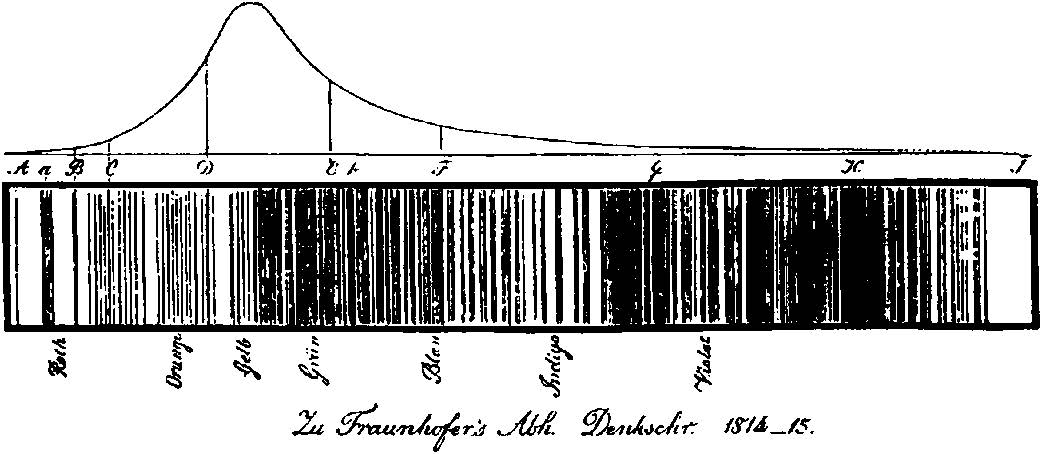
\includegraphics[width=1\textwidth]{figures/intro/Fraunhofer_lines.jpg}}{}{\label{fig:Fraunhofer_lines_old}}
    \vfill
    \Subfigure[0.7]{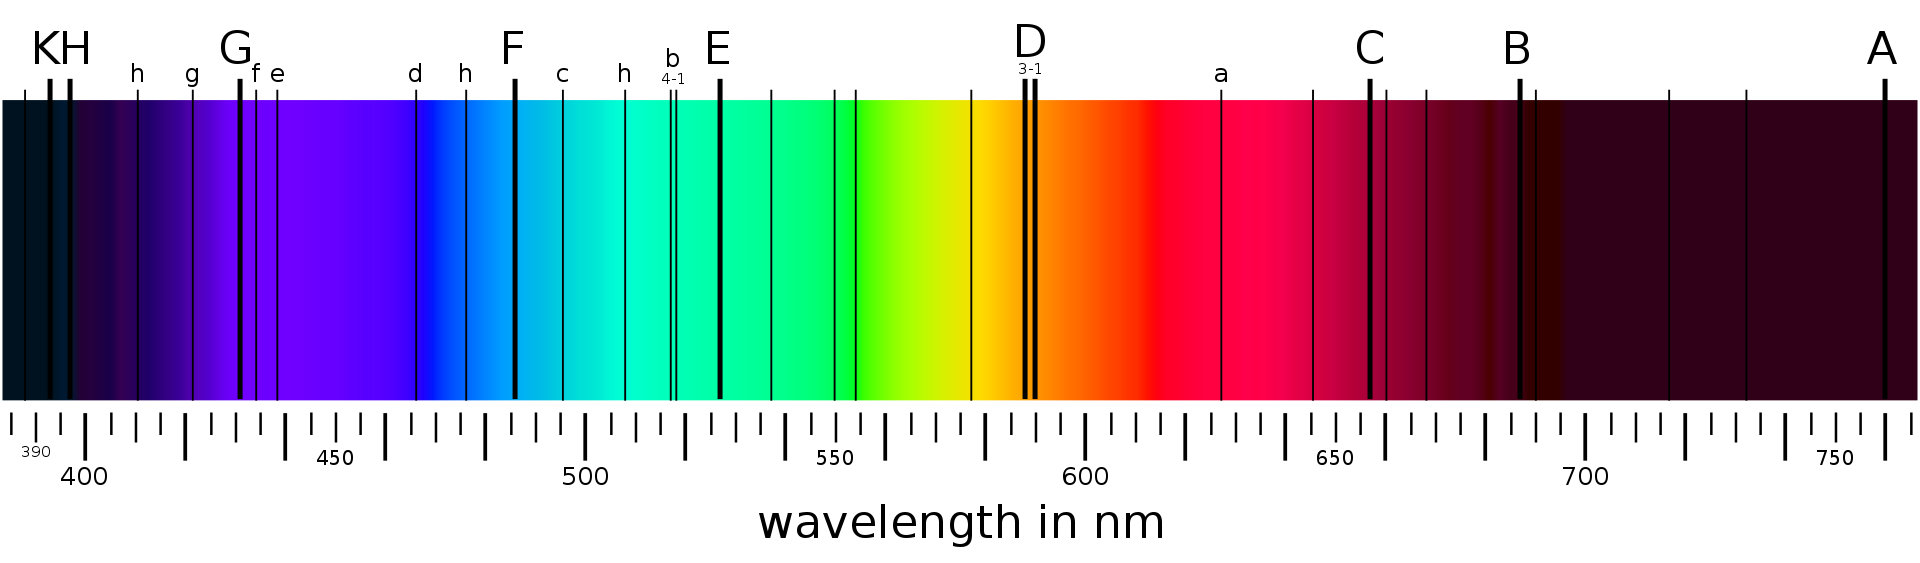
\includegraphics[width=1\textwidth]{figures/intro/Fraunhofer_lines_modern.png}}{}{\label{fig:Fraunhofer_lines_modern}}
    \vfill
    \caption{The optical spectrum of the sunlight. (a) is the original recorded spectrum (Credit: \citet{fraunhofer_first_1817}) while (b) is the same visible spectrum but coloured, from 380 nm to 710 nm (Credit: Wikimedia Commons).} 
    \label{fig:Fraunhofer_lines}
\end{figure}

\citet{fraunhofer_first_1817} used one of the first optics (the same optics that made parallax measurements possible see above) built in 1814 to reflect a ray of sunshine from a slit into a shutter onto a whitewashed wall. 
He noticed that the Sun's light was not a continuous spectrum of colours as observed by Newton \cite{newton_new_1993} 
(see Figure \ref{fig:Fraunhofer_lines}) but a series of dark lines. These lines would later become known as Fraunhofer 
lines. Fraunhofer investigated these lines further and began to record precise positions and intensities 
carefully. As a result, Fraunhofer recorded the first-ever high-resolution astronomical spectrum.
% As shown in Figure \ref{fig:Fraunhofer_lines}, in addition to the rainbow's distinctive colours, which have been observed since Newton \cite{newton_new_1993}, he noticed numerous dark lines. He meticulously recorded the precise wavelength of each dark line, now referred to as Fraunhofer lines, and assigned letters to the strongest ones. As a result, Fraunhofer recorded the first-ever high-resolution astronomical spectrum.

However, he could not determine the origin of the dark patterns he saw. When he conducted a similar experiment using light from the nearby red star Betelgeuse, he discovered that the dark lines he had observed before had significantly altered. Fraunhofer concluded that most of those characteristics were somehow connected to the nature of the object he was examining.

Nearly 45 years later, Gustav Kirchhoff and Robert Bunsen's \cite{kirchhoff_chemical_1860} (1860) experiments helped to understand Fraunhofer's observations. They investigated the colour of the light emitted as metals burned. In certain conditions, they discovered, the wavelength of the produced light matched the Fraunhofer lines. These experiments demonstrated that the atomic constitution of the Sun is the origin of the observation of the Fraunhofer lines. 

\subsection{Beyond stars}
Until the mid-20th century, in the interstellar medium (ISM), the formation and stability of molecules and the efficiency of chemical reactions were assumed to be impossible. The intense radiation and high-energy particles present in space, as well as the extremely low densities (at maximum reaching $10^6 - 10^7$ \percc) and temperatures ($<10$ K) \cite{harju_detection_2008}, were believed to prevent the formation and survival of molecules. For comparison, on Earth global average temperature is around $\sim 298$ K and the number density (atmosphere) amounts to $\sim 10^{19}$ \percc. Therefore, it was generally believed that most matter in space would appear in the form of atoms or amorphous dust grains rather than individual molecules.

\begin{figure}[!htb]
    \centering
    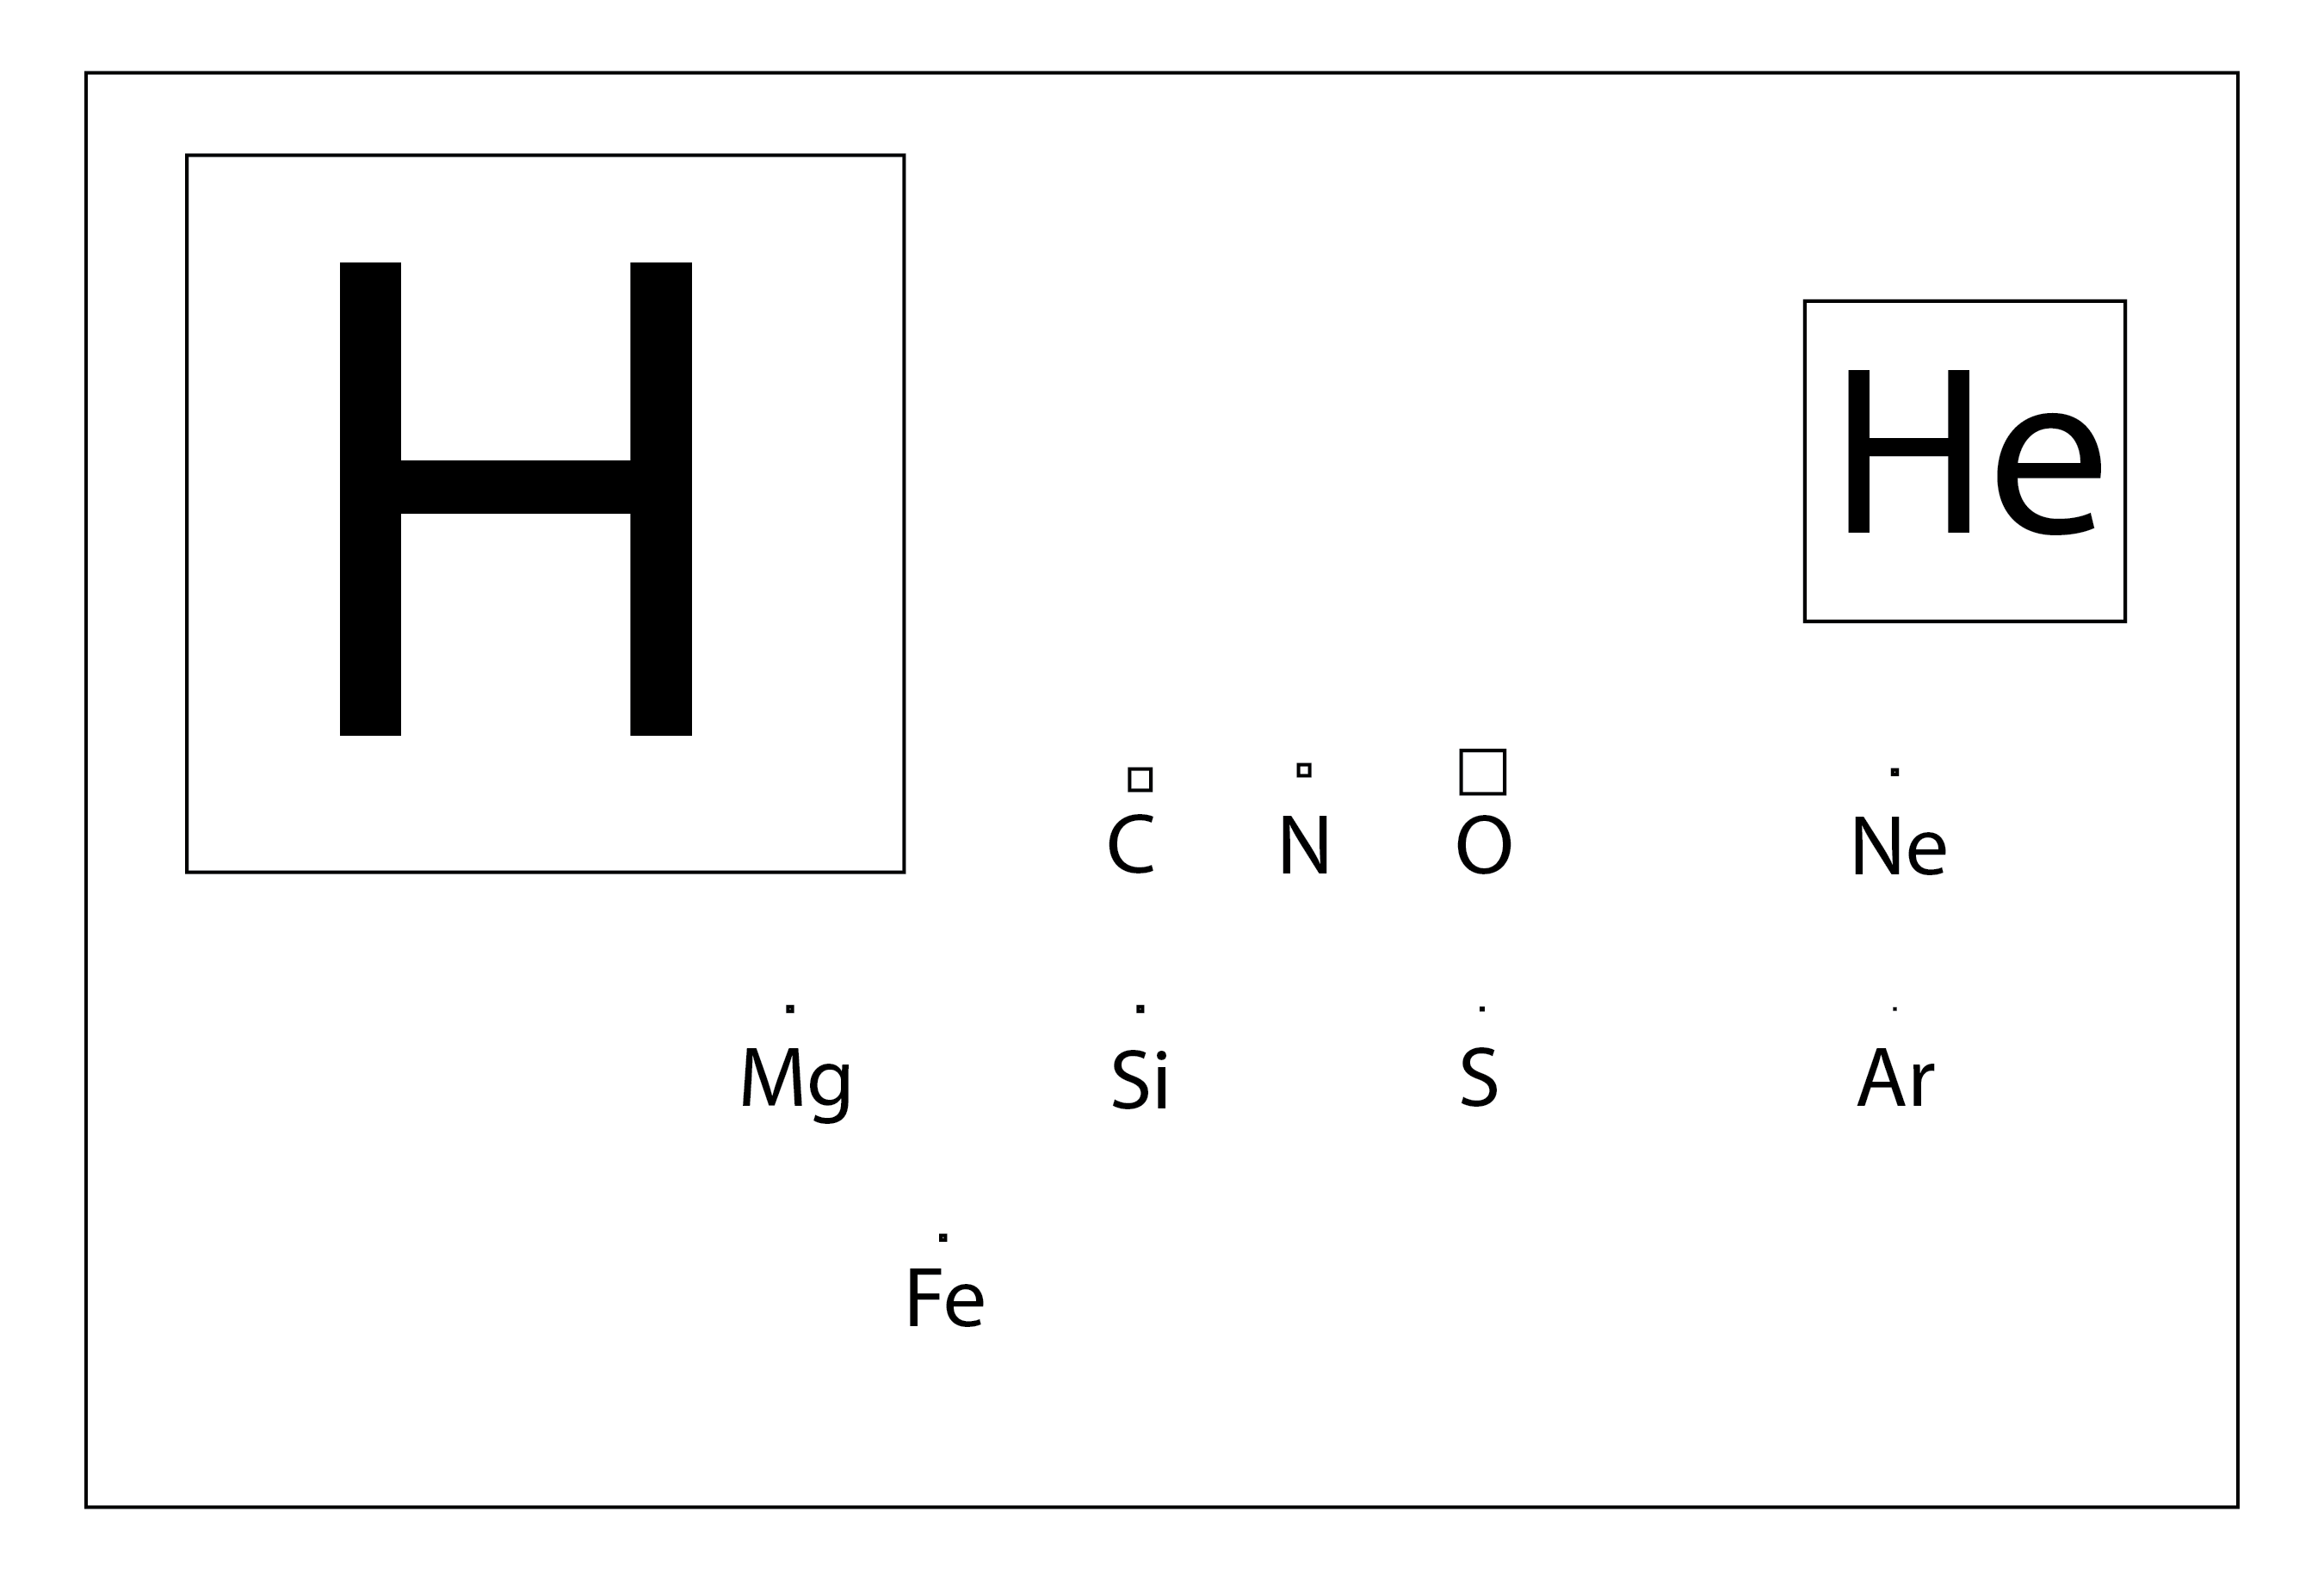
\includegraphics[width=0.6\textwidth]{figures/intro/astro-periodic-table.png}
    \caption{The Astronomer's Periodic Table, as it is referred to. This figure represents the elements by boxes with areas corresponding to their cosmic abundances. Figure adapted from \citet{mccall_optical_2005}.}
    \label{fig:astrochemistry-astro-periodic-table}
\end{figure}

Most astrophysical environments possess very low densities of gases. However, even if densities are high, H and He are 
the primary elements accessible for chemistry (see Figure \ref{fig:astrochemistry-astro-periodic-table}), which was 
thought to limit the complexity of potential chemical reactions significantly. Fortunately, the emergence of 
telescopes, detectors, and spectrometers operating in the radio, infrared (IR), and ultraviolet (UV)/visible regions of 
the electromagnetic spectrum proved this consideration incorrect. Indeed, low densities and extreme temperatures (both 
high and low) in space frequently constrain chemistry, but the vast quantities of matter and long timescale compensate 
for it. Interstellar space represents a unique laboratory in which fundamental molecular processes can be investigated 
under conditions distinctly different from Earth's.

In the following sections, a brief introduction is given to the discovery of molecules in space and the laboratory 
spectroscopic techniques that allow us to study molecular ions under interstellar conditions.
